\documentclass[11pt]{article}
\usepackage[T1]{fontenc}
\usepackage[utf8]{inputenc}
\usepackage{mathpazo}
\usepackage{lmodern}\renewcommand{\rmdefault}{ppl}
\usepackage[margin=1in,headheight=14pt]{geometry}
\usepackage{xcolor}
\usepackage{amsmath,amssymb}
\usepackage{booktabs}
\usepackage{xltabular}
\usepackage{array}
\usepackage{enumitem}
\usepackage{fancyhdr}
\usepackage{titlesec}
\usepackage{listings}
\usepackage[most]{tcolorbox}
\usepackage{tikz}
\usetikzlibrary{arrows.meta,positioning,shapes.geometric}
\usepackage{xurl}
\usepackage[colorlinks=true,linkcolor=atlasblue,urlcolor=atlasblue]{hyperref}

\definecolor{atlasblue}{HTML}{1F4E79}
\definecolor{atlasteal}{HTML}{14776E}
\definecolor{atlasorange}{HTML}{B85C00}
\definecolor{atlasred}{HTML}{B3261E}
\definecolor{codebg}{HTML}{F3F4F6}
\definecolor{boxline}{HTML}{9AA3AD}
\definecolor{accentfill}{HTML}{E3EEF8}

\titleformat{\section}{\Large\bfseries\color{atlasblue}}{\thesection}{0.6em}{}
\titleformat{\subsection}{\large\bfseries\color{atlasblue}}{\thesubsection}{0.6em}{}
\titlespacing*{\section}{0pt}{18pt}{8pt}
\titlespacing*{\subsection}{0pt}{12pt}{5pt}

\pagestyle{fancy}
\fancyhf{}
\fancyhead[L]{\small\textcolor{atlasblue}{\textbf{Atlas v3.1}} -- 20-Hour Build Plan}
\fancyhead[R]{\small CodeRED: Orion}
\fancyfoot[C]{\small\thepage}
\renewcommand{\headrulewidth}{0.4pt}

\setlist{itemsep=2pt,topsep=4pt}
\setlength{\parindent}{0pt}
\setlength{\emergencystretch}{3em}
\setlength{\parskip}{5pt}
\renewcommand{\arraystretch}{1.25}

\newcommand{\code}[1]{\texttt{\detokenize{#1}}}
\newcommand{\verify}{\textbf{[VERIFY]}}
\newcommand{\cb}{$\square$\ }

\lstdefinestyle{sql}{
  language=SQL, basicstyle=\ttfamily\footnotesize, backgroundcolor=\color{codebg},
  keywordstyle=\color{atlasblue}\bfseries, commentstyle=\color{gray}\itshape,
  stringstyle=\color{atlasteal}, frame=single, rulecolor=\color{boxline},
  breaklines=true, columns=fullflexible, keepspaces=true, upquote=true,
  morekeywords={TIMESTAMPTZ,TEXT,BOOLEAN,BIGINT,NUMERIC,DOUBLE,PRECISION,MATERIALIZED,LATERAL,REFERENCES,INTERVAL,WITH,CROSS,HAVING,EXISTS}
}

\newtcolorbox{callout}[2][atlasblue]{colback=#1!4,colframe=#1,fonttitle=\bfseries,title=#2,arc=2pt,boxrule=0.8pt,left=6pt,right=6pt}

\newcolumntype{L}[1]{>{\raggedright\arraybackslash}p{#1}}
\newcolumntype{Y}{>{\raggedright\arraybackslash}X}

\definecolor{fixgreen}{HTML}{14776E}
\newcommand{\fix}[1]{\textcolor{fixgreen}{\textbf{[#1]}}}
\begin{document}

%================ TITLE ================
\begin{titlepage}
\thispagestyle{empty}
\vspace*{3.2cm}
{\fontsize{46}{50}\selectfont\bfseries\color{atlasblue} Atlas\par}
\vspace{0.4cm}
{\LARGE Parametric flood protection for Houston\par}
\vspace{0.5cm}
{\large Fast cash in the first 72 hours, triggered by public gauge data, settled on Solana, priced on Tiger Data\par}
\vspace{0.8cm}
{\color{atlasblue}\rule{\linewidth}{0.8pt}}
\vspace{0.8cm}

{\large\bfseries 20-Hour Build Plan \textemdash{} Version 3.1\par}
\vspace{0.3cm}
CodeRED: Orion \quad | \quad Tracks: Overall, Pitch, Environment, Solana, Tiger Data, Vultr, GoDaddy\par
Team: Jesse (chain, product, hosting) and Ezekiel ``Zeke'' (data, risk); TypeScript and Python only (no Rust)\par
As of October 10, 2026, Hour 4 (5:00 pm CDT)\par
\vspace{1cm}

\begin{callout}{The one-sentence pitch}
Maria rents in Meyerland. When her bayou crosses flood stage, \$500 lands on her phone before the water goes down. That pays for a hotel, food and a missed shift in the first 72 hours, when nothing else pays.
\end{callout}
{\small The bayou is named on stage only after the data confirms it triggers in the replay window. Brays Bayou is preferred because Meyerland sits on it.\par}

\vfill
{\small Assumptions: a team of two, a 20-hour build inside a 24-hour clock that started at 1:00 pm CDT on October 10, devnet only, no custom Solana program. \verify{} items must be checked by Gate G1. Tags such as \fix{V3} point to the v3.1 fix list; tags such as [F7] are v3 fixes, kept.\par}
\end{titlepage}

\tableofcontents
\newpage

%================ CHANGES ================
\section*{Changes from v3}
\addcontentsline{toc}{section}{Changes from v3}

v3.1 keeps the v3 design and fixes the gaps found in its audit and while building the chain side. The chain service, payout bot and dashboard are built to this plan and tested end to end (section 0). The remaining work is the engine, devnet, hosting and the phone test.

{\small
\begin{xltabular}{\linewidth}{@{}l L{4.8cm} Y L{1.2cm}@{}}
\toprule
\# & v3 gap & v3.1 fix & Sec. \\
\midrule
\endhead
\multicolumn{4}{@{}l}{\textcolor{atlasred}{\textbf{Would break a gate or the demo}}} \\
V1 & Code and \code{docs/api.md} used v2 names while v3 renamed tables, fields, statuses, routes and the Memo prefix & v3 names adopted everywhere; \code{docs/api.md} is the single source of truth & 4.2 \\
V2 & Evidence time format undefined across languages (JavaScript adds milliseconds, Python writes \code{+00:00}); no test vector & \code{event_time} is the event's \code{opened_at}, formatted with exact code in both languages; test vector in \code{docs/evidence.md} & 8.7 \\
V3 & Reconciliation fails from run 2: reset only tops up, so premiums accumulate in the vault while the ledger restarts & Reconcile per run against opening balances read from \code{GET /}\allowbreak\code{chain/}\allowbreak\code{balances} at Start & 7.8 \\
V4 & Purchases happen before Start, but every ledger row needs a run & Movements outside a running run are booked to run \code{session} & 7.7 \\
V5 & Flow B co-signed whatever the client posted, so a buyer could zero the premium & Server stores the message hash it built; submit co-signs only on an exact match & 8.3 \\
V6 & aUSD name and symbol impossible on a classic SPL mint without Metaplex & Cut; the phone view is the money moment & 8.1 \\
V7 & Sales could stay frozen between runs & No run running means sales open & 7.9 \\
\multicolumn{4}{@{}l}{\textcolor{atlasorange}{\textbf{High}}} \\
V8 & True-up never runs on-chain in the demo (pool is large, so $f_\text{int}=1$) & One rehearsal with \code{FORCE_F_INT=0.6} on devnet; already passed on a local validator & 5, 12 \\
V9 & Person A carried data, pricing, ledger, reconciliation and all hosting & Hosting, Caddy, domain and deploys move to Jesse, whose code is done & 4.1 \\
V10 & Ledger entries and accounts undefined (``SQL functions agreed in Hour 1'') & Entry table fixed; chain service writes, engine reads; \code{investors} account added & 7.7 \\
V11 & No endpoint for the current run and clock & \code{GET /}\allowbreak\code{replay/}\allowbreak\code{status} added & 4.2 \\
V12 & \code{payout_intents} could not tell ``expired'' from ``in flight'' after a restart & Adds \code{last_}\allowbreak\code{valid_}\allowbreak\code{block_}\allowbreak\code{height}, \code{attempts}, \code{event_id}, \code{owner}, \code{gauge_id} & 6.2, 8.6 \\
V13 & Who marks a storm \code{trued_up} was unstated & The bot, once every true-up confirms & 7.5 \\
V14 & Policy activity judged at ``the run clock'', which moves while the bot works & Judged at the event's \code{opened_at} & 6.5 \\
\multicolumn{4}{@{}l}{\textcolor{atlasblue}{\textbf{Consistency}}} \\
V15 & Section 9 still described Next.js & Web is Vite + React; Next.js notes removed & 9 \\
V16 & Names dropped from the title; banner needs the gauge name & Names restored; \code{/policies} returns \code{gauge_name} and \code{last_payout} & 9.2 \\
V17 & Late start: plan adopted at Hour 4 & Timeline re-based from Hour 4.5; G2 moves to Hour 6.5; upgrades cut to one & 5 \\
\bottomrule
\end{xltabular}
}

%================ STATUS ================
\section*{0\quad Status at Hour 4}
\addcontentsline{toc}{section}{0\quad Status at Hour 4}

\textbf{Built and tested (Jesse).} Chain service, payout bot and dashboard, on a local validator with the devnet Squads program cloned (the devnet faucet refused the build machine).

{\small
\begin{xltabular}{\linewidth}{@{}L{3.6cm} Y@{}}
\toprule
Area & Result \\
\midrule
Policy token & NonTransferable + MetadataPointer + TokenMetadata + PermanentDelegate on one mint; create 985 bytes, purchase 670 of 1,232; name and status \code{ACTV} $\rightarrow$ \code{PAID} $\rightarrow$ \code{ACTV} \\
Purchase & Flow A and Flow B both work; a tampered Flow B transaction (premium set to 0) is refused \\
Abuse limits & Second reservation per wallet refused; non-allowlisted wallet refused; rate limit at 5 per minute; reset refused without the token or via a proxy \\
Storm payouts & $f_\text{int}=0.6$: interim 300 to three policies; $f_\text{fin}=1.0$: true-up 200 each; storm \code{trued_up} \\
Crash recovery & A lost payout intent was expired and rebuilt; paid exactly once \\
Ledger & Every entry sums to zero; float 2,000 $-$ 1,500 = 500 matched the chain \\
Reset and run 2 & Float refilled by minting; policies back to \code{ACTV}; the same policies paid again \\
Evidence & Python-written preimage accepted by the bot; identical test-vector hash in both languages \\
Phone view & ``+\$500 $\bullet$ PAID $\bullet$ Brays Bayou'' appeared live on a confirmed payout \\
\bottomrule
\end{xltabular}
}

\textbf{Not done.} Engine (schema, ingestion, events and storms, pricing, FastAPI); devnet setup; hosting and domain; Phantom phone test; G2.

%================ 1 PRODUCT ================
\section{Product summary and scope}

Atlas pays a fixed sum to every covered household near a Houston bayou gauge within minutes of that gauge crossing flood stage. No claim form, no adjuster.

\subsection{The pitch, led by a person}
Maria rents in Meyerland. When her bayou crosses flood stage, \$500 lands on her phone before the water goes down. That pays for a hotel, food and a missed shift in the first 72 hours, when nothing else pays. Keep the technology out of the first 30 seconds. Name the bayou only after it is confirmed as a demo gauge [F22].

\subsection{The problem}
US flood insurance runs mostly through the federal program, which has a waiting period before cover starts and claims that take weeks or months. Many Houston renters and homeowners have no flood cover at all. In the first 72 hours people need cash for a hotel, a car, food and lost wages.

\subsection{What Atlas does}
Atlas sells a small policy tied to the nearest stream gauge. If that gauge crosses a set flood level during the term, the policyholder gets a fixed payout (for example \$500). In a storm big enough to strain the pool, part is paid immediately and the rest when the storm closes [F7]. Atlas does not pay for property damage and does not replace flood insurance.

\subsection{How each sponsor technology is used}
{\small
\begin{xltabular}{\linewidth}{@{}L{2.8cm} Y@{}}
\toprule
Sponsor & Use \\
\midrule
Tiger Data & Gauge history and live readings as hypertables; continuous aggregates; columnstore compression; event and storm state; pricing from correlated historical-year scenarios; the money ledger; replay engine; simulated 2,000-policy book \\
Solana & aUSD test stablecoin; non-transferable Token-2022 policies with on-chain metadata; atomic purchase; Squads multisig vault; payout bot with intent records; Memo evidence with a canonical hash; catastrophe bond token. Optional: Solana Pay QR or Blink \\
Vultr & Hosts the engine, chain service, bot and dashboard over HTTPS \\
GoDaddy Registry & Domain for the hosted site \\
\bottomrule
\end{xltabular}
}

\subsection{Tracks entered}
Best Overall, Best Pitch/Demo, Best Environment Hack, Best Use of Solana, Best Use of Tiger Data, Best Use of Vultr, Best Domain Name from GoDaddy Registry.

\begin{callout}[atlasorange]{Side-track rule [F24]}
Read the Vultr and GoDaddy Registry rules now. Side-track work is capped at 1 hour total beyond hosting the site and pointing the domain. Confirm on Devpost that one project can enter all seven tracks.
\end{callout}

\subsection{In scope}
6 to 10 gauges with cached history and a live poller; pricing with confidence bands and a correlated capital charge; atomic purchase; storm-level payouts with interim and true-up; ledger-based pool accounting with per-run reconciliation; bond token with NAV; a time-shifted Harvey replay that runs back to back; a hosted, authenticated dashboard with a phone view.

\subsection{Out of scope}
Mainnet, real money, a custom Solana program, KYC, a native mobile app, rainfall triggers, property-level flood modelling, cash-out to bank accounts, aUSD token metadata \fix{V6}, and any claim to be a licensed insurance product.

%================ 2 ARCHITECTURE ================
\section{System architecture}

Every money movement is a ledger row and a transaction on chain, and the two reconcile after every run [F2] \fix{V3}.

\begin{center}
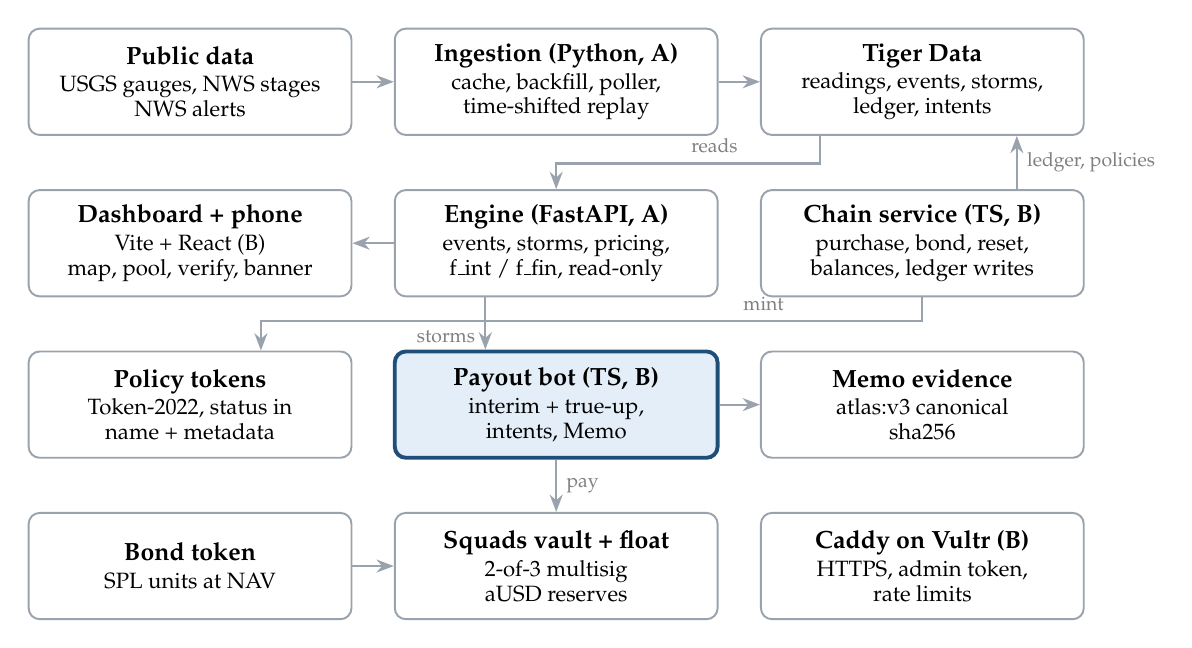
\begin{tikzpicture}[
  box/.style={draw=boxline, rounded corners=4pt, minimum width=4.1cm, minimum height=1.35cm, align=center, font=\small, line width=0.7pt},
  key/.style={box, draw=atlasblue, fill=accentfill, line width=1.4pt},
  arr/.style={-{Stealth[length=2.2mm]}, draw=boxline, line width=0.8pt},
  lbl/.style={font=\scriptsize\color{gray}}
]
\def\cx{4.65} \def\ry{2.05}
\node[box] (pub) at (0,0) {\textbf{Public data}\\[-1pt]{\footnotesize USGS gauges, NWS stages}\\[-2pt]{\footnotesize NWS alerts}};
\node[box] (ing) at (\cx,0) {\textbf{Ingestion (Python, A)}\\[-1pt]{\footnotesize cache, backfill, poller,}\\[-2pt]{\footnotesize time-shifted replay}};
\node[box] (tig) at (2*\cx,0) {\textbf{Tiger Data}\\[-1pt]{\footnotesize readings, events, storms,}\\[-2pt]{\footnotesize ledger, intents}};
\node[box] (web) at (0,-\ry) {\textbf{Dashboard + phone}\\[-1pt]{\footnotesize Vite + React (B)}\\[-2pt]{\footnotesize map, pool, verify, banner}};
\node[box] (eng) at (\cx,-\ry) {\textbf{Engine (FastAPI, A)}\\[-1pt]{\footnotesize events, storms, pricing,}\\[-2pt]{\footnotesize f\_int / f\_fin, read-only}};
\node[box] (svc) at (2*\cx,-\ry) {\textbf{Chain service (TS, B)}\\[-1pt]{\footnotesize purchase, bond, reset,}\\[-2pt]{\footnotesize balances, ledger writes}};
\node[box] (pol) at (0,-2*\ry) {\textbf{Policy tokens}\\[-1pt]{\footnotesize Token-2022, status in}\\[-2pt]{\footnotesize name + metadata}};
\node[key] (bot) at (\cx,-2*\ry) {\textbf{Payout bot (TS, B)}\\[-1pt]{\footnotesize interim + true-up,}\\[-2pt]{\footnotesize intents, Memo}};
\node[box] (memo) at (2*\cx,-2*\ry) {\textbf{Memo evidence}\\[-1pt]{\footnotesize atlas:v3 canonical}\\[-2pt]{\footnotesize sha256}};
\node[box] (bond) at (0,-3*\ry) {\textbf{Bond token}\\[-1pt]{\footnotesize SPL units at NAV}};
\node[box] (vault) at (\cx,-3*\ry) {\textbf{Squads vault + float}\\[-1pt]{\footnotesize 2-of-3 multisig}\\[-2pt]{\footnotesize aUSD reserves}};
\node[box] (caddy) at (2*\cx,-3*\ry) {\textbf{Caddy on Vultr (B)}\\[-1pt]{\footnotesize HTTPS, admin token,}\\[-2pt]{\footnotesize rate limits}};
\draw[arr] (pub) -- (ing);
\draw[arr] (ing) -- (tig);
\draw[arr] ([xshift=-1.3cm]tig.south) -- ++(0,-0.35) -| node[lbl, pos=0.2, above] {reads} (eng.north);
\draw[arr] ([xshift=1.2cm]svc.north) -- node[lbl, right] {ledger, policies} ([xshift=1.2cm]tig.south);
\draw[arr] (eng) -- (web);
\draw[arr] ([xshift=-0.9cm]eng.south) -- node[lbl, left, pos=0.75] {storms} ([xshift=-0.9cm]bot.north);
\draw[arr] (bot) -- (memo);
\draw[arr] (bot) -- node[lbl, right] {pay} (vault);
\draw[arr] (bond) -- (vault);
\draw[arr] (svc.south) -- ++(0,-0.3) -| node[lbl, pos=0.12, above] {mint} ([xshift=0.9cm]pol.north);
\end{tikzpicture}
\end{center}

\subsection{Data flow for one storm}
\begin{enumerate}
\item The poller or replay streamer writes readings with \code{event_time}, \code{wall_time}, \code{source} and \code{run_id} [F9].
\item At Start, the engine records opening balances from \code{GET /}\allowbreak\code{chain/}\allowbreak\code{balances} \fix{V3}.
\item The engine opens an \emph{event} for a gauge after two consecutive accepted readings at or above \code{trigger_ft}, if that gauge has no open event in this run [F8]. It latches the value and writes the canonical preimage and hash [F14][F15] \fix{V2}.
\item The first event in a run opens a \emph{storm} and sets $f_\text{int}$. Later events join the open storm [F7].
\item The bot re-hashes the preimage, then pays every \code{ACTV} policy on that gauge in force at the event's \code{opened_at} \fix{V14} the interim amount $f_\text{int} B$. Each payment is signed, recorded as an intent, then sent [F12].
\item Each interim payment writes a Memo, sets the policy name and status to \code{PAID} in the same transaction, and writes a ledger entry.
\item An event closes after 72 hours of event time continuously below trigger. The storm closes when all its events close, or when the replay ends; the engine sets $f_\text{fin}$.
\item The bot pays the true-up $(f_\text{fin}-f_\text{int})B$ to every interim-paid policy, if positive, then marks the storm \code{trued_up} \fix{V13}.
\item Reconciliation: opening balances plus the run's ledger rows equal the balances now \fix{V3}.
\end{enumerate}

%================ 3 PREFLIGHT ================
\section{Pre-flight checklist (remaining items)}

\textbf{Jesse (B), now:}
\begin{itemize}[label=\cb]
\item Devnet SOL for the treasury from faucet.solana.com (GitHub login), or sent by Zeke. Then the setup in \code{chain/README.md} on devnet; commit \code{chain/}\allowbreak\code{state/}\allowbreak\code{devnet.json}.
\item Vultr instance; Caddy; GoDaddy Registry domain pointed at the IP, with the \code{sslip.io} hostname as fallback [F18].
\item Phone: Phantom in Testnet Mode, funded, screen lock off; phone view URL on the home screen.
\item Read the Vultr, GoDaddy and Devpost multi-track rules [F24].
\end{itemize}
\textbf{Zeke (A), now:}
\begin{itemize}[label=\cb]
\item Tiger Cloud service; TimescaleDB version for the columnstore API [F19]; connection string to Jesse for the server's \code{.env}.
\item Shared \code{ADMIN_TOKEN} generated and stored outside the repo [F6].
\end{itemize}
{\raggedright Already done: monorepo layout, \code{@solana/web3.js} pinned to 1.x, \code{docs/api.md}, \code{docs/evidence.md}, aUSD and Squads scripts, Token-2022 test.\par}

%================ 4 ROLES ================
\section{Team roles and the API contract}

Zeke owns every number and the database. Jesse owns every transaction, every pixel and the servers they run on \fix{V9}.

\subsection{Roles}
{\small
\begin{xltabular}{\linewidth}{@{}L{3.6cm} Y@{}}
\toprule
Role & Owns \\
\midrule
Person A: data and risk (Zeke) & Tiger schema, ingestion, event and storm logic, $f_\text{int}$ and $f_\text{fin}$, replay and run clock, pricing, scenario set, simulated book, ledger reads and reconciliation, FastAPI (read-only), NWS freeze \\
Person B: chain, product and hosting (Jesse) & Chain service (purchase, bond, reset, balances), all signing, aUSD and policy mints, Squads vault, payout bot, Memo evidence, ledger writes, dashboard and phone view, Vultr, Caddy, domain, deploys, upgrades \\
Shared & Gates, pitch, Q\&A, fallback video, Devpost write-up \\
\bottomrule
\end{xltabular}
}

\begin{callout}[atlasorange]{Language boundary}
Python never builds or signs a Solana transaction. The chain service and the bot are the only processes with signing keys. FastAPI reads Tiger and serves JSON; the chain service writes policy and ledger rows; the bot writes intents and marks storms \code{trued_up}.
\end{callout}

\subsection{API contract (\texttt{docs/api.md} is the source of truth) \fix{V1}}
{\small
\begin{xltabular}{\linewidth}{@{}L{4.6cm} Y L{1cm}@{}}
\toprule
Endpoint & Returns & Owner \\
\midrule
\endhead
\code{GET /}\allowbreak\code{replay/}\allowbreak\code{status} \fix{V11} & \code{{run_id, status, clock}} & A \\
\code{GET /}\allowbreak\code{gauges?}\allowbreak\code{run_}\allowbreak\code{id=} & \code{[{gauge_id, name, lat, lon, trigger_ft, latest_ft, status, demo_ready}]} & A \\
\code{GET /}\allowbreak\code{gauges/}\allowbreak\code{{id}/}\allowbreak\code{series?}\allowbreak\code{run_}\allowbreak\code{id=} & \code{{points: [{event_time, stage_ft}], trigger_ft, rejected_count}} & A \\
\code{GET /}\allowbreak\code{quote?}\allowbreak\code{gauge=}\allowbreak\code{&}\allowbreak\code{payout=}\allowbreak\code{&}\allowbreak\code{run_}\allowbreak\code{id=} & \code{{premium, p_payout, band, k, waiting_days, sales_open, reason}} & A \\
\code{GET /}\allowbreak\code{pool?}\allowbreak\code{run_}\allowbreak\code{id=} & \code{{onchain: {seeded_capital, premiums_in, reserve, bond_capital, float, nav_per_unit, payouts_out, reconciled}, simulated: {policies, worst_year_loss, harvey_loss, reserve_used, bond_used, f_int, f_fin, investor_loss_pct}}} & A \\
\code{GET /}\allowbreak\code{storms?}\allowbreak\code{run_}\allowbreak\code{id=} & \code{[{storm_id, status, f_int, f_fin, events: [{event_id, gauge_id, opened_at, closed_at, value, evidence_hash, preimage}], payouts: [{policy, kind, amount, tx_sig}]}]} & A \\
\code{GET /}\allowbreak\code{stress?}\allowbreak\code{scenario=} & \code{harvey} or \code{worst_year}: \code{{aggregate_loss, reserve_used, bond_used, f_fin, investor_loss_pct}} & A \\
\code{GET /}\allowbreak\code{ledger?}\allowbreak\code{run_}\allowbreak\code{id=} & Ledger rows and totals by account & A \\
\code{POST /}\allowbreak\code{replay/}\allowbreak\code{start}, \code{/replay/reset} & \code{{run_id}}; \code{X-Admin-Token}; start records opening balances; reset calls \code{/chain/reset} & A \\
\code{GET/}\allowbreak\code{POST /}\allowbreak\code{api/}\allowbreak\code{actions/}\allowbreak\code{buy?}\allowbreak\code{gauge=}\allowbreak\code{&}\allowbreak\code{payout=}\allowbreak\code{&}\allowbreak\code{flow=} & Action metadata; then a Flow A (server-signed) or Flow B (unsigned) transaction & B \\
\code{POST /}\allowbreak\code{api/}\allowbreak\code{purchase/}\allowbreak\code{submit} & Flow B: co-signs only a message-hash match \fix{V5} & B \\
\code{POST /}\allowbreak\code{api/}\allowbreak\code{bond/}\allowbreak\code{deposit}, \code{/api/bond/submit} & Wallet signs first; server co-signs, sends, writes the ledger entry & B \\
\code{GET /}\allowbreak\code{policies?}\allowbreak\code{owner=} & \code{[{policy_mint, gauge_id, gauge_name, payout, status, paid_amount, last_payout}]} \fix{V16} & B \\
\code{GET /}\allowbreak\code{chain/}\allowbreak\code{balances} & \code{{vault, float, bond_units, ausd_supply, at}} \fix{V3} & B \\
\code{POST /}\allowbreak\code{chain/}\allowbreak\code{reset} & Localhost only, \code{X-Admin-Token}; refill, statuses, reservations & B \\
\bottomrule
\end{xltabular}
}

%================ 5 TIMELINE ================
\section{Timeline, re-based from Hour 4.5 \fix{V17}}

Hour 0 was 1:00 pm CDT, October 10; the deadline is Hour 24. The plan was adopted at Hour 4, so by the late-start rule the lost time comes out of the upgrade block. Jesse's code is done, which frees his hours for devnet, hosting and the phone.

\begin{center}
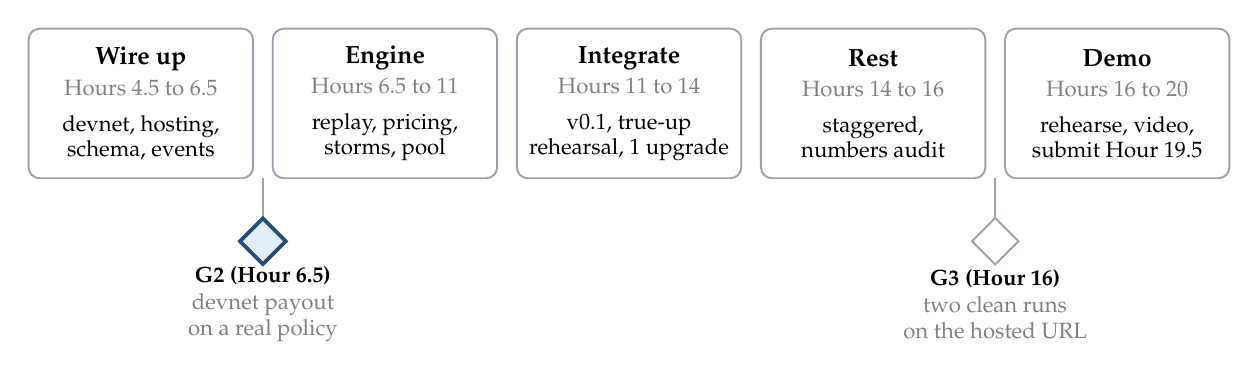
\begin{tikzpicture}[
  band/.style={draw=boxline, rounded corners=4pt, minimum width=2.85cm, minimum height=1.9cm, align=center, font=\small, line width=0.7pt},
  gmark/.style={diamond, draw=boxline, line width=0.7pt, minimum size=0.6cm, inner sep=0pt},
  keymark/.style={gmark, draw=atlasblue, fill=accentfill, line width=1.3pt},
  glbl/.style={align=center, font=\footnotesize}
]
\node[band] at (0,0) {\textbf{Wire up}\\{\footnotesize\color{gray} Hours 4.5 to 6.5}\\[2pt]{\footnotesize devnet, hosting,}\\[-2pt]{\footnotesize schema, events}};
\node[band] at (3.1,0) {\textbf{Engine}\\{\footnotesize\color{gray} Hours 6.5 to 11}\\[2pt]{\footnotesize replay, pricing,}\\[-2pt]{\footnotesize storms, pool}};
\node[band] at (6.2,0) {\textbf{Integrate}\\{\footnotesize\color{gray} Hours 11 to 14}\\[2pt]{\footnotesize v0.1, true-up}\\[-2pt]{\footnotesize rehearsal, 1 upgrade}};
\node[band] at (9.3,0) {\textbf{Rest}\\{\footnotesize\color{gray} Hours 14 to 16}\\[2pt]{\footnotesize staggered,}\\[-2pt]{\footnotesize numbers audit}};
\node[band] at (12.4,0) {\textbf{Demo}\\{\footnotesize\color{gray} Hours 16 to 20}\\[2pt]{\footnotesize rehearse, video,}\\[-2pt]{\footnotesize submit Hour 19.5}};
\draw[draw=boxline, line width=0.7pt] (1.55,-0.95) -- (1.55,-1.45);
\node[keymark] at (1.55,-1.75) {};
\node[glbl] at (1.55,-2.55) {\textbf{G2 (Hour 6.5)}\\{\color{gray}devnet payout}\\{\color{gray}on a real policy}};
\draw[draw=boxline, line width=0.7pt] (10.85,-0.95) -- (10.85,-1.45);
\node[gmark] at (10.85,-1.75) {};
\node[glbl] at (10.85,-2.55) {\textbf{G3 (Hour 16)}\\{\color{gray}two clean runs}\\{\color{gray}on the hosted URL}};
\end{tikzpicture}
\end{center}

\begin{callout}{Gates}
\textbf{G1 (now, overdue):} every \verify{} item answered or its fallback in \code{docs/}\allowbreak\code{decisions.md}, including Phantom Flow A. \textbf{G2 (Hour 6.5):} Zeke's minimal insert script [F17] opens a storm on devnet; the bot pays a real policy; ledger and chain agree. \textbf{G3 (Hour 16, freeze):} on the hosted URL, start, run, reset, run again, twice in a row, no code changes, reconciliation green after each run.
\end{callout}

{\small
\begin{xltabular}{\linewidth}{@{}L{1.5cm} Y Y@{}}
\toprule
Hours & Zeke (data and risk) & Jesse (chain, product, hosting) \\
\midrule
\endhead
4.5 to 6.5 & Tiger schema (6.2); gauges with real site numbers, datum and channel check [F11]; cache Harvey window; event open logic; preimage per \code{docs/evidence.md} (check the test vector); minimal insert script that opens a storm with $f_\text{int}$ & Devnet SOL and setup scripts; Vultr, Caddy, domain or \code{sslip.io}; deploy chain service, bot and web; Phantom Flow A test; precreate policies on demo gauges once Zeke names them \\
\midrule
\multicolumn{3}{@{}p{\linewidth}@{}}{\textcolor{atlasteal}{\textbf{G2 (Hour 6.5)}}: if it fails, cut scope now.} \\
\midrule
6.5 to 9 & Full replay streamer with time shift; event close; storm close and $f_\text{fin}$; \code{/replay/status}, \code{/start} (opening balances), \code{/reset} (calls \code{/chain/reset}) & Point web at the real engine endpoint by endpoint; reset end to end; reconciliation badge from \code{/pool} \\
9 to 11 & Pricing, bootstrap band, historical-year scenarios and $k$; simulated book; stress; NWS freeze with \code{replay_alerts}; admin token on FastAPI & Bond capital deposit on devnet; backup policy per demo wallet [F21]; rate limits and allowlist checked on the hosted URL \\
11 to 12 & \multicolumn{2}{L{11.2cm}}{Integration and food. Start, reset, start on the hosted URL. Tag \code{v0.1}.} \\
12 to 14 & \code{/}\allowbreak\code{docs/}\allowbreak\code{numbers.sql}; reconciliation check script & True-up rehearsal with \code{FORCE_F_INT=0.6} \fix{V8}; one upgrade only: Solana Pay QR (Flow A) or none; verify page on real data \\
14 to 16 & \multicolumn{2}{L{11.2cm}}{Staggered rest: Zeke rests 14 to 15 while Jesse polishes the phone view; Jesse rests 15 to 16 while Zeke runs the numbers audit.} \\
\midrule
\multicolumn{3}{@{}l}{\textcolor{atlasteal}{\textbf{G3 (Hour 16, feature freeze)}}} \\
\midrule
16 to 18 & Slides: pricing, correlated capital, stress & Two rehearsals each of the 90-second and 4-minute scripts; fallback video \\
18 to 19.5 & README numbers section & Devpost page, screenshots, tracks, address list \\
19.5 to 24 & \multicolumn{2}{L{11.2cm}}{Submitted. Sleep in shifts; reset and one full run 20 minutes before judging.} \\
\bottomrule
\end{xltabular}
}

\begin{callout}[atlasorange]{Rule for the whole build}
Blocked for 45 minutes: say so out loud and switch to the fallback (section 12). Already cut by the late start: Switchboard, Squads spending limit, Blink unless Flow A passes and time allows.
\end{callout}

%================ 6 DATA ================
\section{Data layer: Tiger Data}

\subsection{Sources and checks}
\begin{itemize}
\item \textbf{USGS legacy WaterServices:} instantaneous stage and annual peaks. Being retired (see Sources); cache everything and never call it on stage.
\item \textbf{USGS new API:} use for the live poller if the legacy service is degraded.
\item \textbf{NWS flood stages} set \code{trigger_ft} \verify{}; \textbf{NWS alerts} drive the live sales freeze (7.9) \verify{}.
\item \textbf{Cache rule:} every raw response is written to \code{/data/cache/} before parsing.
\end{itemize}
\textbf{Gauge selection:} 6 to 10 gauges on major bayous with live data, at least 20 years of peaks and data through Harvey. Read from the stored data which cross \code{trigger_ft} in the replay window; set \code{demo_}\allowbreak\code{ready =}\allowbreak\code{ true} on four of them [F22].

\textbf{Comparability check [F11]:} for each gauge, read the datum history and channel projects. Price only from the comparable record and note the decision in \code{gauges.record_}\allowbreak\code{note}.

\subsection{Schema}
Engine tables (Zeke). The chain tables \code{policy_pool} and \code{payout_intents} are in \code{chain/}\allowbreak\code{sql/}\allowbreak\code{001_}\allowbreak\code{chain_}\allowbreak\code{tables.sql}.
\begin{lstlisting}[style=sql]
CREATE TABLE gauge_readings (
  event_time TIMESTAMPTZ NOT NULL,                 -- (possibly shifted) hydrologic time
  wall_time  TIMESTAMPTZ NOT NULL DEFAULT now(),   -- when the row was written
  gauge_id TEXT NOT NULL, stage_ft DOUBLE PRECISION, discharge_cfs DOUBLE PRECISION,
  source TEXT NOT NULL,                            -- 'usgs' | 'replay'
  run_id TEXT NOT NULL DEFAULT 'live',
  rejected BOOLEAN NOT NULL DEFAULT false
);
SELECT create_hypertable('gauge_readings', by_range('event_time'));
CREATE UNIQUE INDEX ON gauge_readings (gauge_id, event_time, source, run_id);

CREATE TABLE gauges (
  gauge_id TEXT PRIMARY KEY, name TEXT, lat DOUBLE PRECISION, lon DOUBLE PRECISION,
  trigger_ft DOUBLE PRECISION, nws_flood_ft DOUBLE PRECISION,
  record_start INT, record_note TEXT, feed_pubkey TEXT, demo_ready BOOLEAN DEFAULT false
);
CREATE TABLE annual_peaks (gauge_id TEXT, water_year INT, peak_stage_ft DOUBLE PRECISION,
  peak_time TIMESTAMPTZ, PRIMARY KEY (gauge_id, water_year));

CREATE TABLE runs (run_id TEXT PRIMARY KEY, source TEXT NOT NULL,
  started_wall TIMESTAMPTZ NOT NULL, shift INTERVAL, clock TIMESTAMPTZ,
  status TEXT NOT NULL,                             -- running | done | reset
  opening_vault NUMERIC, opening_float NUMERIC);    -- V3: from GET /chain/balances

CREATE TABLE storms (storm_id TEXT PRIMARY KEY, run_id TEXT NOT NULL,
  opened_at TIMESTAMPTZ NOT NULL, closed_at TIMESTAMPTZ,
  f_int NUMERIC, f_fin NUMERIC, status TEXT NOT NULL); -- open | closed | trued_up (bot)

CREATE TABLE gauge_events (
  event_id TEXT PRIMARY KEY, run_id TEXT NOT NULL, storm_id TEXT NOT NULL,
  gauge_id TEXT NOT NULL, opened_at TIMESTAMPTZ NOT NULL, closed_at TIMESTAMPTZ,
  latched_value DOUBLE PRECISION NOT NULL, feed_pubkey TEXT, feed_slot BIGINT,
  preimage TEXT NOT NULL, evidence_hash TEXT NOT NULL);
CREATE UNIQUE INDEX one_open_event ON gauge_events (run_id, gauge_id) WHERE closed_at IS NULL;

CREATE TABLE policies (
  policy_mint TEXT PRIMARY KEY, owner TEXT NOT NULL, gauge_id TEXT REFERENCES gauges,
  payout_usd NUMERIC NOT NULL, premium_usd NUMERIC NOT NULL,
  starts_at TIMESTAMPTZ NOT NULL, ends_at TIMESTAMPTZ NOT NULL,
  status CHAR(4) NOT NULL,                          -- ACTV | PAID | EXPD
  paid_amount NUMERIC NOT NULL DEFAULT 0, demo BOOLEAN NOT NULL DEFAULT false);

CREATE TABLE sim_policies (sim_id BIGINT PRIMARY KEY, gauge_id TEXT REFERENCES gauges,
  payout_usd NUMERIC, premium_usd NUMERIC);

CREATE TABLE ledger (                               -- written by the chain side (V10)
  wall_time TIMESTAMPTZ NOT NULL DEFAULT now(), run_id TEXT NOT NULL,
  entry_id TEXT NOT NULL, account TEXT NOT NULL, amount NUMERIC NOT NULL,
  memo TEXT, tx_sig TEXT);
SELECT create_hypertable('ledger', by_range('wall_time'));

CREATE TABLE replay_alerts (run_id TEXT, gauge_id TEXT, starts_at TIMESTAMPTZ,
  ends_at TIMESTAMPTZ, kind TEXT);

-- Chain side (V12): payout_intents adds last_valid_block_height, attempts,
-- event_id, owner, gauge_id; see chain/sql/001_chain_tables.sql.
\end{lstlisting}

\subsection{Continuous aggregates and columnstore}
Unchanged from v3: \code{gauge_hourly} grouped by \code{bucket,}\allowbreak\code{ gauge_}\allowbreak\code{id,}\allowbreak\code{ source,}\allowbreak\code{ run_}\allowbreak\code{id} with \code{materialized_}\allowbreak\code{only =}\allowbreak\code{ false}; columnstore policy after 7 days with the old compression API as fallback [F19]. History charts read \code{gauge_hourly}; the live replay chart reads \code{gauge_readings} for the current run.

\subsection{Event logic}
One rule for pricing and the contract [F8]: an event opens after two consecutive accepted readings at or above \code{trigger_ft}; it closes once the gauge has stayed below \code{trigger_ft} for 72 hours of event time. At most one open event per gauge per run. The open and close queries are unchanged from v3. At the end of a replay the streamer closes all open events and the storm at the run clock. The data-quality guard marks jumps \code{rejected = true}; the gauge page shows the count.

\subsection{Run clock and replay}
\begin{itemize}
\item \textbf{Run clock:} \code{now()} for a live run; the \code{event_time} of the last reading written for a replay. Grep for \code{now()} and \code{Date.now()} at Hour 10.
\item \textbf{Window and speed:} 48 hours before the first demo gauge crosses to 24 hours after the last peak; seconds per reading = \code{REPLAY_}\allowbreak\code{SECONDS /}\allowbreak\code{ count} [F20].
\item \textbf{Shift:} \code{event_}\allowbreak\code{time =}\allowbreak\code{ original_}\allowbreak\code{time + (started_}\allowbreak\code{wall - window_}\allowbreak\code{start)}.
\item \textbf{Policy activity:} a policy is eligible for an event if \code{starts_}\allowbreak\code{at <=}\allowbreak\code{ opened_}\allowbreak\code{at < ends_}\allowbreak\code{at} \fix{V14}. Policies run 365 days, so the future-dated replay stays inside the term.
\end{itemize}

\subsection{Reset}
\code{POST /}\allowbreak\code{replay/}\allowbreak\code{reset} (admin token): stop the streamer and mark the run \code{reset}; call \code{POST /}\allowbreak\code{chain/}\allowbreak\code{reset} with the run id (refill vault and float to the snapshot by minting aUSD, demo policies to \code{ACTV} on-chain and in Tiger, release reservations, \code{seeded} ledger rows); then reconcile. Holders keep the aUSD they received; reset mints new test aUSD, so total supply grows. Say so if asked.

%================ 7 PRICING ================
\section{Pricing and capital model}

\subsection{Event frequency}
$\hat\lambda^\text{peak}_g = N^\text{peak}_g / T_g$ from annual peaks, and $\hat\lambda^\text{iv}_g$ from instantaneous data with the contract's open/close rule. Price with the higher of the two [C3]; say which on the slide.

\subsection{Premium}
\[ P(\text{payout}) = 1 - e^{-\hat\lambda_g t}, \qquad \mathbb{E}[L] = B\,(1 - e^{-\hat\lambda_g t}), \qquad \pi = \mathbb{E}[L](1+\theta) + c\,k. \]
Interim plus true-up never exceed $B$. Bootstrap 2,000 times for a 5th to 95th percentile band.

\subsection{Correlated capital and $k$}
Each historical year is one scenario across all gauges: $S_y = \sum_{i} B_i\,\mathbf{1}\{\text{peak}_{g(i),y} \ge \text{trigger}_{g(i)}\}$. Required capital $K = \max(\max_y S_y,\ S_\text{Harvey}) - \bar S$, a worst-observed-year standard, not a modelled tail. Each policy's share is $k_i = K B_i / \sum_j B_j$.

\subsection{Waterfall}
Each premium is split once: expenses $e\pi$; bond coupon $ck$, which accrues into NAV (no distributions in the demo); the rest to reserve $R$. Losses hit $R$, then bond capital $C$, then the pay factor.
\[ \text{NAV}_t = \frac{C_0 - \text{losses absorbed}_t + \text{coupons accrued}_t}{\text{units outstanding}}. \]

\subsection{Storm payouts: interim and true-up}
\[ f_\text{int} = \min\Big(1,\ \frac{A}{B\,N_\text{risk}}\Big), \qquad f_\text{fin} = \min\Big(1,\ \frac{A}{B\,N_\text{trig}}\Big) \ \ge f_\text{int}, \]
where $A$ is available funds ($R + C$) at storm open, $N_\text{risk}$ the active policies on all gauges in the at-risk set, and $N_\text{trig}$ those whose gauges triggered by storm close. The engine writes $f_\text{int}$ when the storm opens and $f_\text{fin}$ when it closes; the bot never computes them. For the true-up rehearsal the engine honours \code{FORCE_F_INT} \fix{V8}.

\subsection{Two pool panels}
On-chain (devnet): seeded capital labelled ``seeded'', not premiums [F26]; premiums; reserve; bond capital; float; NAV; reconciliation badge. Simulated book: 2,000 policies; worst-year and Harvey losses; layer use; $f_\text{int}$ and $f_\text{fin}$; investor loss.

\subsection{Ledger entries \fix{V4} \fix{V10}}
Written by the chain side; each entry sums to zero; the engine reads them and owns the economic split (expenses, coupon, which layer absorbs a loss). Movements outside a running run go to run \code{session}.

{\small
\begin{xltabular}{\linewidth}{@{}L{5.2cm} Y@{}}
\toprule
Movement & Rows \\
\midrule
Policy purchase & \code{holders} $-\pi$, \code{premiums} $+\pi$ \\
Bond deposit & \code{investors} $-D$, \code{bond} $+D$ \\
Payout (interim or true-up) & \code{float} $-x$, \code{holders} $+x$ \\
Reset refill of the vault & \code{seeded} $-x$, \code{reserve} $+x$ \\
Reset refill of the float & \code{seeded} $-y$, \code{float} $+y$ \\
Vault to float by proposal & \code{reserve} $-z$, \code{float} $+z$ \\
\bottomrule
\end{xltabular}
}

\subsection{Reconciliation per run \fix{V3}}
At \code{/replay/start} the engine stores \code{opening_vault} and \code{opening_float} from \code{GET /}\allowbreak\code{chain/}\allowbreak\code{balances}. After the run, for the vault (\code{premiums}, \code{reserve}, \code{bond} rows) and for the float (\code{float} rows): opening balance + sum of this run's rows = \code{GET /}\allowbreak\code{chain/}\allowbreak\code{balances} now. Absolute totals are never compared, because reset only tops up.

\subsection{Underwriting rules}
\begin{itemize}
\item Waiting period 7 days; demo mode sets 0, and the demo says so.
\item \textbf{Sales freeze:} live mode reads NWS alerts for the gauge's point; replay mode reads \code{replay_alerts} for the running run (a flood watch from 24 hours of event time before the first crossing). \textbf{When no run is running, sales are open} \fix{V7}. The live API is never consulted in demo mode.
\item One policy per wallet per gauge; one active reservation per wallet.
\end{itemize}

%================ 8 SOLANA ================
\section{Solana layer (Jesse)}

All signing lives in the chain service and the bot [F16]. Built and tested; the remaining work is devnet, the phone and one optional upgrade.

\subsection{aUSD}
Classic SPL Token mint, 6 decimals, 1,000,000 to the treasury. No token metadata \fix{V6}: Phantom will show an unnamed token; the phone view is the money moment. Policies use Token-2022 and aUSD the classic Token program; every associated token account is derived with the right program.

\subsection{Policy tokens}
Supply 1, 0 decimals; NonTransferable, MetadataPointer (to itself), TokenMetadata, and PermanentDelegate (burn at expiry only). Status is a fixed-width code in both the name (\code{Atlas Policy ACTV}, \code{Atlas Policy PAID}) and the \code{status} field, with 256 bytes of rent pre-funded [F13]. Fields: \code{policy_id}, \code{gauge_id}, \code{status}, \code{terms_hash}, and \code{uri} to the terms JSON. About 10 pre-created mints per demo gauge.

\subsection{Atomic purchase}
One transaction: create the buyer's Token-2022 account; \code{transferChecked} the premium to the vault; \code{mintTo} one policy; remove the mint authority. The mint is reserved for 2 minutes; one active reservation per wallet.

{\small
\begin{xltabular}{\linewidth}{@{}L{3.4cm} Y@{}}
\toprule
Flow & How \\
\midrule
A (preferred) & The server partially signs as mint authority; the wallet signs as fee payer and sends. Works for the Buy button, Solana Pay and Blinks. \\
B (fallback) & The server returns the transaction unsigned and stores the hash of its message. The wallet signs; \code{/}\allowbreak\code{api/}\allowbreak\code{purchase/}\allowbreak\code{submit} co-signs only if the posted message hash matches exactly \fix{V5}, then sends. Blinks are dropped. \\
\bottomrule
\end{xltabular}
}
\textbf{Phone test (G1):} run Flow A from the phone in Phantom Testnet Mode against the hosted service. If Phantom rejects or warns, set \code{PURCHASE_FLOW=b} and \code{VITE_}\allowbreak\code{PURCHASE_}\allowbreak\code{FLOW=}\allowbreak\code{b} and record decision \#11.

\subsection{Pool: Squads multisig}
2-of-3 Squads v4; the vault is a PDA, so its aUSD account uses \code{allowOwnerOffCurve =}\allowbreak\code{ true}; time lock about 60 seconds in demo mode. The bot float (2,000 aUSD) is pool money held by the bot; it is refilled by reset or by one proposal.

\subsection{Payout bot}
Per storm: interim $f_\text{int}B$ to each \code{ACTV} policy on a triggered gauge after an on-chain check (holder, status \code{ACTV}, gauge); true-up $(f_\text{fin}-f_\text{int})B$ after close; storm marked \code{trued_up} \fix{V13}. Interim transactions carry the transfer, the Memo and the \code{PAID} name and status together. If the float is short, the bot warns once and waits.

\subsection{Idempotency}
\begin{enumerate}
\item \code{intent_}\allowbreak\code{id =}\allowbreak\code{ sha256(policy_}\allowbreak\code{mint|}\allowbreak\code{storm_}\allowbreak\code{id|}\allowbreak\code{kind)}; skip if confirmed or in flight.
\item Sign the transaction; the signature is known before sending.
\item Insert the intent with \code{tx_sig}, \code{last_}\allowbreak\code{valid_}\allowbreak\code{block_}\allowbreak\code{height} and status \code{signed} \fix{V12}. Only then send.
\item On every tick, first settle unsettled intents: confirmed $\rightarrow$ ledger and policy rows exactly once; failed or blockhash expired $\rightarrow$ \code{expired}, rebuilt as a new attempt; otherwise wait.
\end{enumerate}

\subsection{Evidence \fix{V2}}
\begin{lstlisting}[basicstyle=\ttfamily\footnotesize,backgroundcolor=\color{codebg},frame=single,rulecolor=\color{boxline},breaklines=true,columns=fullflexible]
atlas|v3|{gauge_id}|{value}|{event_time}|{run_id}|{storm_id}|{event_id}|{feed}|{slot}
\end{lstlisting}
\begin{itemize}
\item \code{value}: latched triggering value, exactly 2 decimals. \code{event_time}: the event's \code{opened_at}, UTC, whole seconds, trailing \code{Z}. Python: \texttt{strftime("\%Y-\%m-\%dT\%H:\%M:\%SZ")}; TypeScript: \code{toISOString()} without milliseconds. \code{feed}, \code{slot}: Switchboard values or \code{-}.
\item SHA-256 of the UTF-8 preimage, lowercase hex; Memo \code{atlas:v3:<hash>}. The preimage is stored in \code{gauge_events}; the bot re-hashes it before paying; the verify page re-hashes it again.
\item Test vector: \code{atlas|}\allowbreak\code{v3|}\allowbreak\code{08074500|}\allowbreak\code{31.46|}\allowbreak\code{2026-10-11T03:15:00Z|}\allowbreak\code{run-7|}\allowbreak\code{run-7-s1|}\allowbreak\code{run-7-e3|}\allowbreak\code{-|}\allowbreak\code{-} hashes to:\\ {\small\code{a3bf1d54bf92482a546d48927da5801cc8452da55dee080956c8ce7222bf3642}}
\end{itemize}

\subsection{Bond token}
Classic SPL mint. Deposits always use wallet-first signing: the investor signs, the server co-signs on \code{/api/bond/submit}, sends and writes the ledger entry. NAV comes from the ledger (7.4). Redemption is cut.

\subsection{Reset (chain side)}
Localhost only, admin token. Mint aUSD into vault and float up to the snapshot (\code{SNAPSHOT_VAULT}, \code{SNAPSHOT_FLOAT}); set demo policies to \code{ACTV} (name and status, three per transaction); mark them \code{ACTV} with \code{paid_amount = 0} in Tiger; release reservations; write \code{seeded} rows; return balances before and after.

\subsection{Upgrades (after G2, only one)}
Solana Pay QR on the same buy endpoint, only if Flow A passes (1 hour; drop if not working on the phone). Already cut by the late start: Blink, Squads spending limit, Switchboard.

%================ 9 WEB ================
\section{Backend, frontend and hosting}

\subsection{Services}
{\small
\begin{xltabular}{\linewidth}{@{}L{4cm} Y L{1.2cm}@{}}
\toprule
Service & Role & Owner \\
\midrule
FastAPI & Read-only API over Tiger; replay start and reset orchestration; pricing; stress & Zeke \\
Streamer and poller (Python) & Live polling; replay; event and storm ticks & Zeke \\
Chain service (TypeScript) & Purchase, bond, Actions, \code{/chain/reset}, \code{/chain/balances}, \code{/policies} & Jesse \\
Payout bot (TypeScript) & Interim and true-up payouts; intents; Memo & Jesse \\
Web (Vite + React) \fix{V15} & Dashboard and phone view & Jesse \\
\bottomrule
\end{xltabular}
}
All run on one Vultr instance under systemd or pm2, behind Caddy. Keep a full local copy runnable on a laptop.

\subsection{Frontend}
{\small
\begin{xltabular}{\linewidth}{@{}L{2.4cm} Y@{}}
\toprule
Page & Shows \\
\midrule
Map & Gauges coloured normal, near, triggered; demo gauges; storm status; Start and Reset only when the admin token is stored \\
Gauge & Stage over event time with the trigger line and event markers; rejected count; quote with band, $k$ and freeze status; Buy (Flow A or B) \\
Pool & On-chain panel with seeded capital labelled and reconciliation badge; simulated book with $f_\text{int}$ and $f_\text{fin}$; payouts by kind \\
Verify & Payout signature $\rightarrow$ preimage, recomputed hash, Memo hash, match \\
Phone view & One wallet: balance from chain, ``+\$500 $\bullet$ PAID $\bullet$ Brays Bayou'' banner with the transaction link \fix{V16} \\
Admin & Stores the admin token in the demo laptop's browser \\
\bottomrule
\end{xltabular}
}

\subsection{Hosting, security and abuse limits}
\begin{itemize}
\item Caddy terminates HTTPS for the GoDaddy domain; if DNS has not propagated, use the \code{sslip.io} hostname for the Vultr IP.
\item \code{POST /replay/*} and \code{/chain/reset} require \code{X-Admin-Token}; \code{/chain/reset} accepts only direct loopback connections.
\item Buy and bond: 5 requests per minute per IP; demo allowlist (\code{DEMO_WALLETS}); one active reservation per wallet; reservations expire after 2 minutes.
\item Keys only in server environment files: \code{issuer} and \code{treasury} for the chain service, \code{bot} and \code{issuer} for the bot.
\end{itemize}

%================ 10 DEMO ================
\section{Demo script}

The moment that wins: the bayou line turns red and the phone view shows the payout at the same instant.

\textbf{Stage set-up:} map on the laptop; phone view mirrored beside it; admin token loaded; fallback video open; one backup policy already bought on a second demo wallet [F21].

\subsection{90-second version}
{\small
\begin{xltabular}{\linewidth}{@{}L{2.4cm} Y@{}}
\toprule
0:00 to 0:15 & ``Maria rents in Meyerland. Federal flood claims take weeks. She needs money in the first 72 hours.'' \\
0:15 to 0:35 & Tap a demo gauge. Quote: probability, premium, band. Buy on the phone; if it has not confirmed in 10 seconds, switch to the backup wallet. \\
0:35 to 1:10 & Start the replay. The map turns red; the phone view shows ``+\$500 $\bullet$ PAID''. \\
1:10 to 1:30 & Pool page: reserve used, bond absorbs the rest, reconciliation green. ``Priced from decades of gauge data in Tiger Data, settled on Solana in seconds.'' \\
\bottomrule
\end{xltabular}
}

\subsection{4-minute version}
{\small
\begin{xltabular}{\linewidth}{@{}L{2.4cm} Y@{}}
\toprule
0:00 to 0:30 & The gap, told through Maria. One sentence on Atlas. \\
0:30 to 1:15 & A demo gauge. Quote with band and history. Buy on the phone (backup ready). ``Waiting period is off in demo mode.'' \\
1:15 to 2:30 & Replay. Map turns red; payouts land; phone shows PAID. Storm closes: ``everyone in the storm gets the same share.'' Pool: reserve used, NAV drops. \\
2:30 to 3:00 & Verify one payout: preimage, hash, Memo match. \\
3:00 to 3:30 & Numbers: worst-year capital need, simulated interim and true-up factors, Tiger compression ratio. \\
3:30 to 4:00 & Limitations in one breath (basis risk, licensing, cash-out), then the close. \\
\bottomrule
\end{xltabular}
}

\begin{callout}[atlasred]{Demo rules}
Only the four \code{demo_ready} gauges. Press Reset before every judge group and check the reconciliation badge is green. One full run 20 minutes before judging. Never debug in front of judges: switch to the fallback video within 15 seconds.
\end{callout}

%================ 11 QA ================
\section{Judge Q\&A preparation}
{\small
\begin{xltabular}{\linewidth}{@{}L{4.2cm} Y@{}}
\toprule
Question & Answer \\
\midrule
\endhead
Your bot decides to pay. What does the chain add? & Purchase is one atomic transaction, so payment cannot be separated from the policy. Every payout carries a Memo hash of the exact reading it acted on. Solvency and every payout are public. A Solana program enforcing the payout rule is the production step. \\
Is the payout fair in a big storm? & Every triggered policy gets the same interim share at once, sized against all policies that could trigger, and a true-up when the storm closes. Order of crossing does not matter. \\
Which numbers are real? & On-chain panel: real devnet balances, with starting capital labelled seeded. Simulated panel: a 2,000-policy book, labelled. \\
How do you know the books are right? & Every money movement is a ledger row. Each run's opening balances plus its ledger rows equal the on-chain balances afterwards; the badge shows it. \\
How does Maria cash out? & In this build she can't. Off-ramps exist through third parties; a production version would partner with one or pay through a card linked to the wallet [F25]. \\
What if the gauge triggers but my street stayed dry? & Basis risk, the core trade-off of parametric cover. Payouts are small and fixed for immediate needs. Rainfall and multi-gauge triggers are next. \\
How did you size capital? & Each historical year is a scenario across all gauges, so correlation is built in. Capital covers the worst observed year above the mean: a worst-year standard, not a modelled 1-in-200. \\
Is your flood history comparable over time? & Datum and channel changes were checked per gauge; pricing uses only the comparable record. \\
Is this legal? & Selling insurance needs a licence; the bond token is likely a security. Atlas is the engine an insurer, city programme or nonprofit would run. \\
Can you fake the oracle? & In this build the bot reads Tiger and the replay is served by our server; we say so. An on-chain oracle is the production path. \\
What stops double payment? & Every payout is signed and recorded before it is sent; a restarted bot settles every recorded signature before building anything new. \\
Why does aUSD supply keep growing? & Reset mints test aUSD to restore the pool between demo runs. In production there is no reset. \\
\bottomrule
\end{xltabular}
}

%================ 12 RISK ================
\section{Risk register, fallbacks and cut order}
{\small
\begin{xltabular}{\linewidth}{@{}L{3.7cm} L{1.4cm} L{3.4cm} Y@{}}
\toprule
Risk & Odds & Switch trigger & Fallback \\
\midrule
\endhead
Devnet faucet refuses & High & No SOL by Hour 5 & faucet.solana.com with GitHub login; Zeke sends SOL; last resort: demo on a local validator, said aloud \\
Engine late for G2 & High & No storm row by Hour 6.5 & Minimal insert script only; pricing numbers from a notebook for slides \\
Phantom rejects Flow A & Medium & Phone test & Flow B; drop the QR upgrade \\
DNS not propagated & Medium & Not resolving by Hour 6 & \code{sslip.io} hostname \\
Reconciliation fails & Medium & Badge red & Fix before G3; check opening balances were recorded at Start \\
True-up path breaks on devnet & Low & Rehearsal & Already passed locally; demo storm uses $f_\text{int}=1$ \\
Running out of time & High & Missed gate & Cut order below \\
Live demo failure & Medium & Anything breaks & Fallback video, 15-second rule \\
Venue network or Vultr fails & Medium & Site unreachable & Local stack, hotspot \\
USGS legacy degraded & Medium & Failed call & New API; else cache only, live poller dropped and said so \\
Tiger Cloud limits & Low & Blocking error & Local Docker TimescaleDB \\
\bottomrule
\end{xltabular}
}

\textbf{Cut order (first cut first):} QR upgrade; GEV fit; verify page; bond deposit flow (seed bond capital by script); true-up beat in the 4-minute script (keep the logic); live poller.

\textbf{Never cut:} time-shifted replay with reset and refill; ledger and reconciliation; admin token; the phone view payout; the map turning red; the pool page; the hosted URL; the backup policy; the fallback video.

%================ 13 LIMITATIONS ================
\section{Limitations of the product}
\begin{itemize}
\item \textbf{Insurance design:} basis risk; fixed benefit for immediate needs only; one payout per term; partial interim payment in a large storm with the rest days later; adverse selection reduced, not removed.
\item \textbf{Data and oracle:} gauges fail in the largest floods; provisional data can be revised after a payout; single source, itself mid-migration at USGS; record comparability shortens usable history; the replay is served by the team on shifted time; the bot decides to pay, and the Memo makes that auditable, not enforced.
\item \textbf{Pricing and capital:} few extreme events and wide bands; non-stationarity; capital set to the worst observed year; catastrophe figures from a simulated book; bond holders can lose most of their principal.
\item \textbf{Legal:} licensed insurer or approved programme required; the bond token is likely a security; disclosure rules apply; payouts depend on a stablecoin.
\item \textbf{Users:} no cash-out; a lost wallet means a lost policy; people in a crisis may distrust an unfamiliar product.
\item \textbf{Hackathon build:} devnet and test money; reset mints new aUSD between runs; aUSD has no name in wallets; waiting period off in demo mode; custodial keys; a hot-wallet float; no code audit.
\end{itemize}

%================ 14 SUBMISSION ================
\section{Submission checklist}
Submit by Hour 19.5; the deadline is 1:00 pm CDT, October 11 (Hour 24).
\begin{itemize}[label=\cb]
\item Hosted URL on the GoDaddy domain (or documented \code{sslip.io}), tested from a phone on mobile data.
\item Admin controls hidden and protected on the public site.
\item Public repository: README with problem, architecture, setup, run, reset and refill, evidence format, limitations.
\item On-chain addresses: aUSD mint, an example policy, multisig and vault, float wallet, bond mint, sample purchase, interim and true-up transactions.
\item Demo video (2 to 3 minutes) with the phone view visible.
\item Slides: Maria, demo, pricing, correlated capital, stress test, Tiger Data usage, Solana usage, limitations, next steps.
\item All seven tracks selected if allowed; each sponsor's usage described separately.
\item \code{/}\allowbreak\code{docs/}\allowbreak\code{numbers.sql} reproduces every number on the slides; reconciliation passes.
\item Reset pressed, one full run, badge green, 20 minutes before judging.
\end{itemize}

%================ 15 ASSUMPTIONS ================
\section{Unverified assumptions (G1, overdue)}
Each needs a yes or its fallback in \code{docs/}\allowbreak\code{decisions.md}. Items already answered on a local validator are marked; recheck them on devnet.
\begin{itemize}[label=\cb]
\item Phantom on the phone accepts Flow A [F3]; Phantom shows the policy name.
\item USGS legacy and new API coverage for the chosen gauges; history depth; datum and channel changes [F11].
\item NWS flood stages and alerts by point.
\item Exact Harvey window, reading count and the four gauges that cross trigger [F20][F22].
\item Token-2022 extensions, name and status updates, purchase under 1,232 bytes (passed locally; recheck on devnet).
\item Squads multisig, vault account and time lock (passed locally with the devnet program cloned; recheck on devnet).
\item Tiger Cloud columnstore API [F19]; free-tier limits; whether the track requires Tiger Cloud.
\item Vultr and GoDaddy track rules; Devpost multi-track entry [F24].
\item Domain resolving, or \code{sslip.io} working with Caddy [F18].
\end{itemize}

\section*{Sources}
\addcontentsline{toc}{section}{Sources}
Carried over from v3 (not re-checked):
\begin{itemize}
\item USGS Water Data APIs (legacy WaterServices retirement and possible degradation): \url{https://www.usgs.gov/tools/usgs-water-data-apis}
\item USGS API decommission notice: \url{https://waterdata.usgs.gov/blog/api-decom-fall-2025/}
\item Circle testnet faucet (devnet USDC limits): \url{https://developers.circle.com/w3s/docs/developer-console-faucet}
\item CodeRED: Orion on Devpost (tracks, rules, deadline): \url{https://codered-orion-ccs.devpost.com/}
\end{itemize}

\end{document}
